\documentclass{beamer}

% \usepackage[english]{babel}
\usepackage[utf8]{inputenc}
\usepackage{float} % per posizionare le figure float opzione H
\usepackage{amsfonts}
\usepackage{amsmath}
\usepackage{amsthm}
\usepackage{amssymb}
\usepackage[ruled,linesnumbered]{algorithm2e} % per gli algoritmi in pseudocodice
\usepackage{listings} % per inserire il codice in C
\usepackage{longtable}
\usepackage{booktabs}
\usepackage{graphicx} % to include images
\usepackage{xspace}
\usepackage{hyperref}
\usepackage[]{xcolor}
% \usepackage{rotating}
\usepackage{dirtree}
\usepackage[hang,small,sc]{caption}

% Codici %
\renewcommand\lstlistingname{Listing}
\renewcommand\lstlistlistingname{Listings}
% END Codici %

% ALIAS %
\newcommand{\dt}{TosKer\xspace}

%TOSKER MODULES
\newcommand{\mdeployer}{\emph{Orchestrator}\xspace}
\newcommand{\mparser}{\emph{TOSCA utility}\xspace}
\newcommand{\msoftware}{\emph{Software manager}\xspace}
\newcommand{\mcontainer}{\emph{Container manager}\xspace}
\newcommand{\mvolume}{\emph{Volume manager}\xspace}
\newcommand{\mdocker}{\emph{Docker interface}\xspace}
\newcommand{\mmanager}{\emph{Managers}\xspace}

%TOSKER TYPES
\newcommand{\tpersistent}{\emph{tosker.\-nodes.\-Container.\-Executable}\xspace}
\newcommand{\tcontainer}{\emph{tosker.\-nodes.\-Container}\xspace}
\newcommand{\tvolume}{\emph{tosker.\-nodes.\-Volume}\xspace}
\newcommand{\timage}{\emph{tosker.\-artifacts.\-Image}\xspace}
\newcommand{\tdockerfile}{\emph{tosker.\-artifacts.\-Dockerfile}\xspace}
\newcommand{\tsoftware}{\emph{tosker.\-nodes.\-Software}\xspace}
% END ALIAS %

% Definition of the colours
\definecolor{codegreen}{rgb}{0,0.6,0}
\definecolor{codegray}{rgb}{0.5,0.5,0.5}
\definecolor{codepurple}{rgb}{0.58,0,0.82}
\definecolor{backcolour}{rgb}{0.95,0.95,0.92}
\definecolor{deepblue}{rgb}{0,0,0.5}
\definecolor{deepred}{rgb}{0.6,0,0}
\definecolor{deepgreen}{rgb}{0,0.5,0}

% Default fixed font does not support bold face
\DeclareFixedFont{\ttb}{T1}{txtt}{bx}{n}{10} % for bold
\DeclareFixedFont{\ttm}{T1}{txtt}{m}{n}{10}  % for normal

% LISTINGS YAML %
\newcommand\YAMLcolonstyle{\color{red}\footnotesize\mdseries}
\newcommand\YAMLkeystyle{\color{black}\footnotesize\bfseries}
\newcommand\YAMLvaluestyle{\color{blue}\footnotesize\mdseries}

\makeatletter

% here is a macro expanding to the name of the language
% (handy if you decide to change it further down the road)
\newcommand\language@yaml{yaml}

\expandafter\expandafter\expandafter\lstdefinelanguage
\expandafter{\language@yaml}
{
  keywords={true,false,null,y,n},
  keywordstyle=\color{darkgray}\bfseries,
  basicstyle=\YAMLkeystyle,                                 % assuming a key comes first
  sensitive=false,
  comment=[l]{\#},
  morecomment=[s]{/*}{*/},
  commentstyle=\color{purple}\ttfamily,
  stringstyle=\YAMLvaluestyle\ttfamily,
  moredelim=[l][\color{orange}]{\&},
  moredelim=[l][\color{magenta}]{*},
  moredelim=**[il][\YAMLcolonstyle{:}\YAMLvaluestyle]{:},   % switch to value style at :
  morestring=[b]',
  morestring=[b]",
  literate =    {---}{{\ProcessThreeDashes}}3
                {>}{{\textcolor{red}\textgreater}}1
                {|}{{\textcolor{red}\textbar}}1
                {\ -\ }{{\mdseries\ -\ }}3,
}

% switch to key style at EOL
\lst@AddToHook{EveryLine}{\ifx\lst@language\language@yaml\YAMLkeystyle\fi}
\makeatother

\newcommand\ProcessThreeDashes{\llap{\color{cyan}\mdseries-{-}-}}

\lstdefinestyle{TOSCA}{
  captionpos=t,
  % abovecaptionskip=0.8\baselineskip,
  belowcaptionskip=0.8\baselineskip,
  keepspaces=true,
  numbersep=5pt,
  xleftmargin=\parindent,
  language=yaml,
  % basicstyle=\ttm,
  basicstyle=\footnotesize\ttfamily,
  commentstyle=\itshape\color{purple!40!black},
  numberstyle=\tiny\color{codegray},
  numbers=left,
  frame=tb,
}
%% END LISTINGS YAML %%


%% LISTING PYTHON %%
\lstdefinestyle{mystyle}{
    % % backgroundcolor=\color{backcolour},
    % commentstyle=\color{codegreen},
    % keywordstyle=\ttb\color{deepblue},
    % numberstyle=\tiny\color{codegray},
    % stringstyle=\color{codepurple},
    % basicstyle=\ttm,
    % breakatwhitespace=false,
    % breaklines=true,
    % keepspaces=true,
    % numbers=left,
    % numbersep=5pt,
    % showspaces=false,
    % showstringspaces=false,
    % showtabs=false,
    % tabsize=2,
    % language=Python
    captionpos=t,
    belowcaptionskip=0.8\baselineskip,
    % abovecaptionskip=1\baselineskip,
    breaklines=true,
    language=Python,
    basicstyle=\ttm,
    otherkeywords={self},             % Add keywords here
    keywordstyle=\ttb\color{deepblue},
    emph={MyClass,__init__},          % Custom highlighting
    emphstyle=\ttb\color{deepred},    % Custom highlighting style
    stringstyle=\color{deepgreen},
    commentstyle=\color{codegray},
    numberstyle=\tiny\color{codegray},
    numbers=left,
    frame=tb,                         % Any extra options here
    showstringspaces=false            %
}

%% END LISTING PYTHON %%


\usepackage{graphicx}
\usepackage{caption}
\usepackage{subcaption}

% \usepackage[backend=bibtex, sorting=nty, style=numeric]{biblatex}
% \addbibresource{../references.bib}

\usetheme{Frankfurt}
\usecolortheme{whale}
% #3778C6
\definecolor{myblue1}{RGB}{55,120,198}
\definecolor{myblue2}{RGB}{37,78,136}
\definecolor{myblue3}{RGB}{0,20,137}
% \definecolor{white}{RGB}{255,255,255}
% \definecolor{black}{RGB}{0,0,0}


\setbeamercolor*{frametitle}{fg=white,bg=myblue2}
\setbeamercolor*{title}{fg=white,bg=myblue2}
\setbeamercolor*{structure}{fg=myblue2}


\title[About Beamer] %optional
{Orchestrating applications with\\ TOSCA and Docker}

% \subtitle{A short story}

\author[lucarin91] % (optional, for multiple authors)
{Luca Rinaldi}

\institute[unipi] % (optional)
{
  {\small University of Pisa}
}

% \logo{\includegraphics[height=1.5cm]{../thesis/style/logo.png}}

\date[2017] % (optional)
{
  {\small June 2017}
}

% \AtBeginSubsection[]
% {
% \begin{frame}{Table of Contents}
% \tableofcontents[
%   currentsection,
%   currentsubsection,
%   sectionstyle=show/shaded,
%   subsectionstyle=show/shaded
% ]
% \end{frame}
% }
\AtBeginSection[]{
  \begin{frame}{Table of Contents}
    \tableofcontents[currentsection]
  \end{frame}
}

\begin{document}
\begin{frame}
  \maketitle
\end{frame}

% \begin{frame}{Table of Contents}
%   \tableofcontents
% \end{frame}

\section{Context}\subsection*{}

  \begin{frame}{Software deployment}
    The execution of all the activities that make a software system available to use.

    Nowadays strictly related to the cloud infrastructure.

    Need of a way to express all the \textbf{requirements} that the application needs to run.
  \end{frame}


\section{Docker}\subsection*{}

  \begin{frame}{Docker}
    \begin{figure}
      
\includegraphics[width=0.8\textwidth]{img/docker.png}
    \end{figure}
    % Docker containers wrap up the software and all the requirements: code, runtime, system tools, system libraries.
    % This guarantees that the software always run in all environment that support Docker.
  \end{frame}

  \begin{frame}{Docker: What?}
    \begin{figure}
      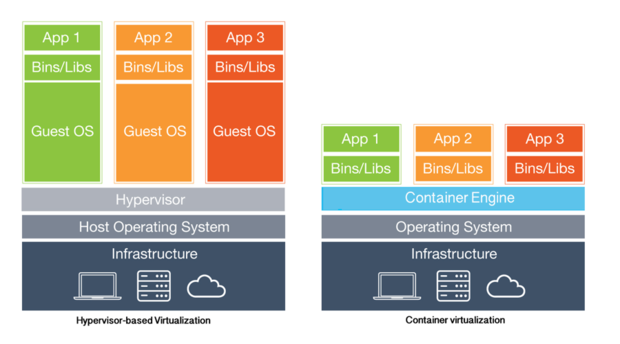
\includegraphics[width=1\textwidth]{img/docker_vs_vm.png}
    \end{figure}
  \end{frame}

  \begin{frame}{Docker: Architecture}
    \begin{figure}
      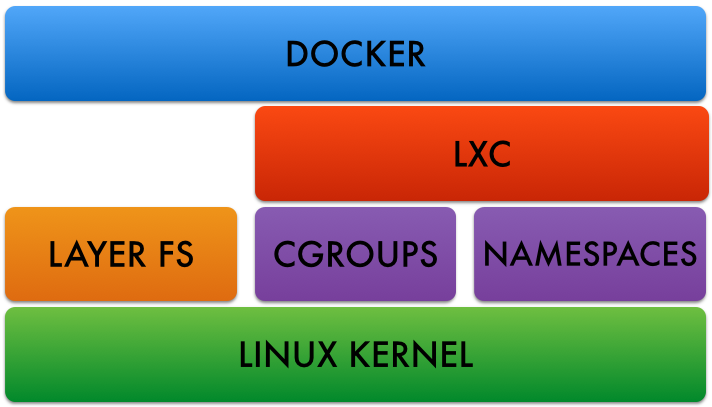
\includegraphics[width=0.8\textwidth]{img/docker_achitecture_crop.png}
    \end{figure}
    \begin{itemize}
      \item LXC %TODO: add spiegazione
      \item LAYER FS
      \item CGROUPS
      \item NAME SPACE
      \item LINUX KERNEL
    \end{itemize}
  \end{frame}

  \begin{frame}{Docker: main comcepts}
    Main concept of the Docker platform
    \begin{itemize}
      \item \texttt{Dockerfile}, a scripts to generate an Image
      \item \texttt{Docker Image}, a LAYER FS archive whit all the data
      \item \texttt{Docker Container}, Running instance of a Docker Image
      \item \texttt{Docker Volume}, a persistent data storage
      \item \texttt{Docker Hub}, a Database of Docker Image open to comunity
    \end{itemize}
  \end{frame}

  \begin{frame}{Docker: pro and cons}

  \end{frame}

\section{TOSCA}\subsection*{}

  \begin{frame}{TOSCA: What?}

  \end{frame}

  \begin{frame}{TOSCA: How?}

  \end{frame}

  \begin{frame}{TOSCA: main concept}

  \end{frame}

  \begin{frame}{TOSCA: problems}

  \end{frame}

\section{TosKer}\subsection*{}

  \begin{frame}{TosKer: what?}

  \end{frame}

  \begin{frame}{TosKer: how?}

  \end{frame}

  \begin{frame}{TosKer: DEMO}

  \end{frame}

  \begin{frame}{TosKer: main advantage}

  \end{frame}

\section{Conclusion and Future works}\subsection*{}

  \begin{frame}{Future works}

  \end{frame}

  \begin{frame}{Conclusions}

  \end{frame}

  \begin{frame}
    \centering
    \Huge Thank You \\
    \bigskip
    \LARGE Q\&A
  \end{frame}
\end{document}
